\documentclass[a4paper,10pt]{article}
\usepackage{amsmath}
\usepackage{graphicx}
% If you want to use Chinese, include the following package
\usepackage{CJKutf8}
\usepackage{color}

\title{CS5321 Numerical Optimization Homework 1}
\author{Due Oct 28}
\date{}
\begin{document}
\maketitle
\begin{enumerate}
 \item (30\%) For a single variable unimodal function $f \in [0, 1]$, we want to find its minimum.  We have introduced the binary search algorithm in the class.  But in each iteration, we need two function evaluations, $f(x_k)$ and $f(x_k+\epsilon)$.  Here is another type of algorithms, called ternary search. Figure \ref{fig1} illustrates the idea.  The initial triplet of $x$ values is $\{x_1, x_2, x_3\}$.   
\begin{figure}[h]
\centering
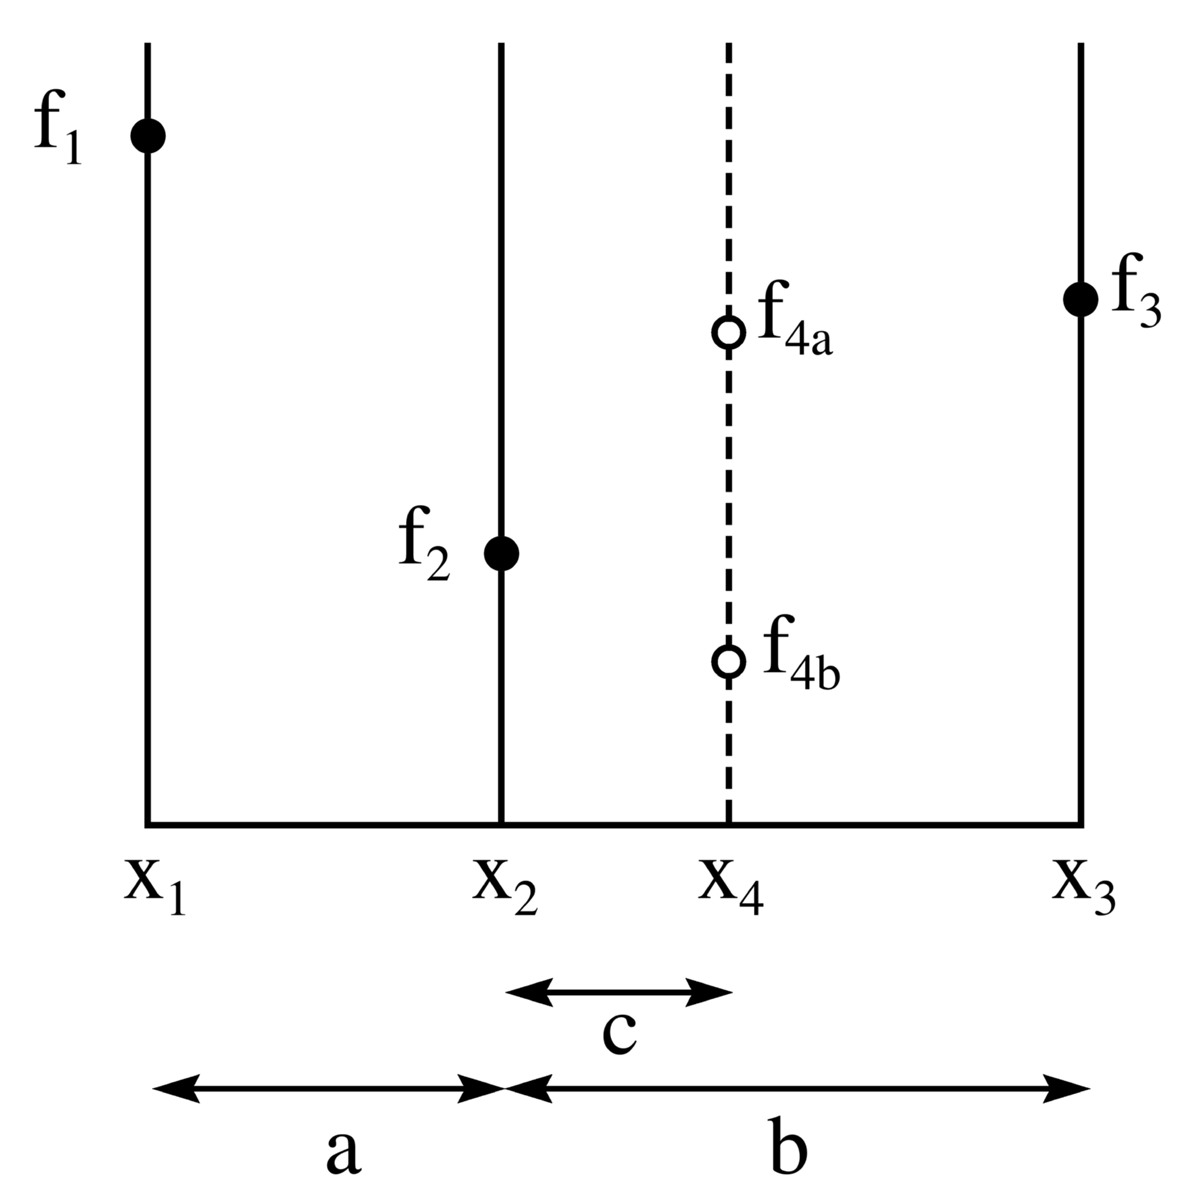
\includegraphics[scale=0.1]{GoldenSectionSearch.png}
\caption{The idea of ternary search.}
\label{fig1}
\end{figure}




\begin{enumerate}
		\item (10\%) For the search direction, show that to find the minimum point, if $f(x_4)=f_{4a}$, the triplet $\{x_1,x_2,x_4\}$ is chosen for the next iteration. If $f(x_4)=f_{4b}$, the triplet $\{x_2, x_4, x_3\}$ is chosen. (Hint: use the property of unimodal.)
		
{\color{blue}
\begin{CJK*}{UTF8}{bsmi}
根據unimodel的性質,$\exists x \in [x_1,x_3]$ 裡面一定有極值,表示只要x往極值移動時,一定為單調遞增或單調遞減\\
反證法:\\
若$f(x_4)= f_{4a}$,假設此函數在$\exists x_m \in [x_4,x_3]$之間有極值,但這就違反了unimodel的定義,因為無法單調遞增或遞減,其不是唯一\\
local minimum。\\
若$f(x_4)= f_{4b}$,假設此函數在$\exists x_m \in [x_1,x_2]$有極值,但這就違反unimodel的性質,因為無法單調遞增或遞減,其不是唯一的local minimum
\end{CJK*}

}
    \item (10\%) For either case, we want these three points keep the same ratio, which means
    $$\frac{a}{b} = \frac{c}{a} = \frac{c}{b-c}.$$
    Show that under this condition, the ratio of $b/a=(\sqrt{5}+1)/2$, which is the golden ratio $\phi$. (So this algorithm is called the \emph{Golden-section search}).
    
{\color{blue} 

\begin{CJK*}{UTF8}{bsmi}
假設 a = b = c = 0 不成立的狀態下\\\\
$$\frac{a}{b} = \frac{c}{a}
\rightarrow c = \frac{a^{2}}{b}$$\\\\

由右邊的等式得出\\\\
$$\frac{c}{a} = \frac{c}{b-c}
\rightarrow  a = b - c $$\\\\

帶入第一條進第二條並通乘$\frac{b}{a^{2}}$
$$\frac{b}{a} = \frac{b^{2}}{a^{2}} - 1 
\rightarrow (\frac{b}{a})^{2} - \frac{b}{a} - 1 = 0 $$
再根據上面算出來的結果使用公式解得
$$\frac{b}{a} = \frac{1 \pm  \sqrt{5}}{2}$$
又因為 $a$ and $b$ 為長度故相除一定大於零
$$\frac{b}{a} = \frac{1 +  \sqrt{5}}{2}$$
\end{CJK*}

}   
 
    \item (10\%) If we let each iteration of the algorithm has two function evaluations, show the convergence rate of the Golden-section search is  $\phi^{-2}$.  (This means it is faster than the binary search algorithm under the same number of function evaluations.)  
    \end{enumerate}

{\color{blue}

\begin{CJK*}{UTF8}{bsmi}
因為binary search需要目標值與中間元素進行比較,才能進行一次收斂,但ternary search每次收斂都只需要1個點(以這題來說就是$x_4$),這邊將ternary search每次也都帶入2個點

$$\frac{b}{a+b}= \frac{ \frac{b}{a}}{1+\frac{b}{a}}$$
將 $b/a=(\sqrt{5}+1)/2$帶入後可得$$\frac{b}{a+b}=(\sqrt{5}-1)/2$$因此可知每帶一次點可以收斂$\phi^{-1}$($\phi = \frac{b}{a}$),所以收歛兩次等於對其做平方,故得$\phi^{-2}$
\end{CJK*}
}

\item (15\%) Show that Newton's method for single variables is equivalent to build a quadratic model 
$$q(x) = f(x_k) + f'(x_k)(x-x_k) + \frac{f''(x_k)}{2}(x-x_k)^2$$
at the point $x_k$ and use the minimum point of $q(x)$ as the next point.  (Hint: to show the next point $x_{k+1} = x_k -f'(x_k)/f''(x_k)$) 

{\color{blue}

\begin{CJK*}{UTF8}{bsmi}
將其排列成 quadratic model 常見的樣子
$$q(x) = \frac{f''(x_k)}{2}x^2+[f'(x_k)-f''(x_k)x_k]x+[f(x_k)-f'(x_k)x_k+\frac{f''(x_k)}{2}x_k^2]$$
利用配方法,K為常數,不需要完整地寫出來\\
$$q(x) = \frac{f''(x_k)}{2}[x+(\frac{f'(x_k)}{f''(x_k)} - x_k)]^2+ K $$
$$x = x_k - \frac{f'(x_k)}{f''(x_k)}$$
可以獲得最小值$q(x)$,因為平方出來一定為正數,所以讓其為零必定可以獲得最小值
\\

Newton'method定義
$$x_{k+1} = x_k - \frac{f'(x_k)}{f''(x_k)} $$
所以可以從兩者所得出的結論知道,newton method對於單一變數而言就是等同於建立一個 quadratic model
\end{CJK*}

}

\item (15\%) Matrix $A$ is an $n\times n$ symmetric matrix.  Show that  
all $A$'s eigenvalues are positive if and only if $A$ is positive definite. 

{\color{blue}

\begin{CJK*}{UTF8}{bsmi}
當$A$為實對稱矩陣時,$A$可以正交對角化,所以必定存在一個正交矩陣$Q$使得$Q^{T}AQ = D$,D為 diagonal matrix,對角線上的值為A的eigunvalues\\
因為$Q$為正交矩陣,所以其$Q^{-1} = Q^{T}$\\
又
$$A = QDQ^{T}$$
左右通乘$x^{T}x$\\
得
$$x^{T}Ax = x^{T}QDQ^{T}x$$
令
$$y = Q^{T}x$$
$$y^{T} = x^{T}Q$$
得
$$x^{T}Ax = y^{T}Dy$$
$$= \lambda_{1}y_1 + \lambda_{2}y_2 + \lambda_{3}y_3 + ... + \lambda_{n}y_n$$
假設其$\lambda_{i}$皆為正數,且x不會等於 zero vector 所以y也不會是 zero vector ,上面的式子可以得出$x^{T}Ax > 0$,符合正定矩陣的定義,故得證其為正定矩陣//
反之\\
$$Ax = \lambda x$$
同時左右乘$x^{T}$
$$x^{T}Ax = \lambda x^{T}x$$
當左邊的A為正定時,左邊皆為正值(建立在 eigunvector 不等於零)正定的性質$x^{T}Ax > 0$所以右半部一定大於零,且$x^{T}x$可以看成x的norm,所以其 eigunvalue 必定為正
\end{CJK*}

}

  \item (50\%) Consider a function $f(x_1,x_2) = (x_1-x_2)^3+2(x_1-1)^2$. 
   	\begin{enumerate}
    \item Suppose $\vec{x}_0=(1,2)$. Compute $\vec{x_1}$ using the steepest descent step with the optimal step length.

{\color{blue}
partial derivative for $x_1$ 
$$\frac{\partial f(x_1,x_2)}{\partial x_1}=3(x_1-x_2)^2 +4(x_1 -1)$$
partial derivative for $x_2$
$$\frac{\partial f(x_1,x_2)}{\partial x_2}=-3(x_1-x_2)^2$$
so we get  $$\nabla f = \begin{bmatrix}
3(x_1-x_2)^2 +4(x_1 -1) \\-3(x_1-x_2)^2
\end{bmatrix}$$
second derivative for $x_1$ 
$$\frac{\partial^2 f(x_1,x_2)}{\partial x_1^2}=6(x_1-x_2)+4$$
second derivative for $x_2$
$$\frac{\partial^2 f(x_1,x_2)}{\partial x_2^2}=6(x_1-x_2)$$
second derivative for $x_1$ and $x_2$ 
$$\frac{\partial^2 f(x_1,x_2)}{\partial x_1 \partial x_2}=-6(x_1-x_2)$$
so we get $$H = \begin{bmatrix}
6(x_1-x_2)+4&-6(x_1-x_2)\\-6(x_1-x_2)&6(x_1-x_2)
\end{bmatrix}$$
$$\vec{g_0}=\nabla f(1,2)=\begin{bmatrix}
3\\-3
\end{bmatrix}$$
$$\vec{p_0}=-\nabla f(1,2)=\begin{bmatrix}
-3\\3
\end{bmatrix}$$
$$H(1,2)=\begin{bmatrix}
-2&6\\6&-6
\end{bmatrix}$$
$$\alpha=\frac{-\vec{g_0}^T \vec{p_0}}{\vec{p_0}^T H \vec{p_0}}=\frac{-\begin{bmatrix}
3&-3
\end{bmatrix}\begin{bmatrix}
-3\\3
\end{bmatrix}}{\begin{bmatrix}
-3&3
\end{bmatrix}\begin{bmatrix}
-2&6\\6&-6
\end{bmatrix}\begin{bmatrix}
-3\\3
\end{bmatrix}}=-\frac{1}{10}$$
$$\vec{x_1}=\begin{pmatrix}
1\\2
\end{pmatrix}-\frac{1}{10}\begin{pmatrix}
-3\\3
\end{pmatrix}=\begin{pmatrix}
\frac{13}{10}\\\frac{17}{10}
\end{pmatrix}$$
}

    \item What is the Newton's direction of $f$ at $(x_1,x_2)=(1,2)$?  Is it a descent direction?

{\color{blue}
	$$\vec{p_k}=-H_k ^{-1} \vec{g_k}=-\begin{bmatrix}
-2&6\\6&-6
\end{bmatrix}\begin{bmatrix}
3\\-3
\end{bmatrix}=\begin{bmatrix}
0\\-\frac{1}{2}
\end{bmatrix}$$
$H^{-1}$ is not positive definite because of negative eigenvalue.\\
Use Graphing calculator to check whether it get negative eigunvalue. 
In the end, $\vec{p_k}$ is not a descent direction.
   

}

    \item Compute the LDL decomposition of the Hessian of $f$ at $(x_1,x_2)=(1,2)$. (No pivoting)


{\color{blue}
$$H=\begin{bmatrix}
-2&6\\6&-6
\end{bmatrix}
\stackrel{r_{12}(3)}{\longrightarrow}
\begin{bmatrix}
-2&6\\0&12
\end{bmatrix}
\stackrel{c_{12}(3)}{\longrightarrow}
\begin{bmatrix}
-2&0\\0&12
\end{bmatrix}$$
$$=\begin{bmatrix}
1&0\\-3&1
\end{bmatrix}\begin{bmatrix}
-2&0\\0&12
\end{bmatrix}\begin{bmatrix}
1&-3\\0&1
\end{bmatrix}=LDL^T$$

}
    \item Compute the modified Newton step using LDL modification.

{\color{blue} 
\begin{CJK*}{UTF8}{bsmi}
這邊將-2的位置改成+2,使其 diagonal 為正值
$$\hat{H}=L\hat{D}L^T=\begin{bmatrix}
1&0\\-3&1
\end{bmatrix}
\begin{bmatrix}
2&0\\0&12
\end{bmatrix}
\begin{bmatrix}
1&-3\\0&1
\end{bmatrix}=
\begin{bmatrix}
2&-6\\-6&30
\end{bmatrix}$$
$$\vec{p}=-\hat{H}^{-1}\vec{g}=
-\begin{bmatrix}
\frac{5}{4}&\frac{1}{4}\\\frac{1}{4}&\frac{1}{12}
\end{bmatrix}
\begin{bmatrix}
3\\-3
\end{bmatrix}=
\begin{bmatrix}
-3\\-\frac{1}{2}
\end{bmatrix}$$
\end{CJK*}

}
    \item Suppose $\vec{x}_0=(1,1)$ and $\vec{x}_{1}=(1,2)$, and the $B_0=I$. Compute the quasi Newton direction $p_1$ using BFGS.

{\color{blue} 
$$\vec{s_0}=\vec{x_1}-\vec{x_0}=
\begin{bmatrix}
0\\1
\end{bmatrix}$$
$$\vec{y_0}=\nabla f(1,2)-\nabla f(1,1)=
\begin{bmatrix}
3\\-3
\end{bmatrix}$$
since $$B_1=B_0-\frac{B_0\vec{s_0}\vec{s_0}^TB_0}{\vec{s_0}^TB_0\vec{s_0}}+\frac{\vec{y_0}\vec{y_0}^T}{\vec{y_0}^T\vec{s_0}}$$
$$B_1=
\begin{bmatrix}
1&0\\0&1
\end{bmatrix}
-\frac{\begin{bmatrix}
0\\1
\end{bmatrix}
\begin{bmatrix}
0&1
\end{bmatrix}}
{\begin{bmatrix}
0&1
\end{bmatrix}
\begin{bmatrix}
0\\1
\end{bmatrix}}+\frac{\begin{bmatrix}
3\\-3
\end{bmatrix}
\begin{bmatrix}
3&-3
\end{bmatrix}}
{\begin{bmatrix}
3&-3
\end{bmatrix}
\begin{bmatrix}
0\\1
\end{bmatrix}}=
\begin{bmatrix}
-2&3\\3&-3
\end{bmatrix}$$
$$\vec{p_1}=-B_1^{-1}\vec{g_1}=-B_1^{-1}\cdot\nabla f(\vec{x_1})=-\begin{bmatrix}
1&1\\1&\frac{2}{3}
\end{bmatrix}
\begin{bmatrix}
3\\-3
\end{bmatrix}=
\begin{bmatrix}
0\\-1
\end{bmatrix}$$

}

    \end{enumerate}


\end{enumerate}



\end{document}
